\documentclass[journal,12pt,twocolumn]{IEEEtran}
%
\usepackage{setspace}
\usepackage{gensymb}
\usepackage{siunitx}
\usepackage{tkz-euclide} 
\usepackage{textcomp}
\usepackage{standalone}
\usetikzlibrary{calc}

%\doublespacing
\singlespacing

%\usepackage{graphicx}
%\usepackage{amssymb}
%\usepackage{relsize}
\usepackage[cmex10]{amsmath}
%\usepackage{amsthm}
%\interdisplaylinepenalty=2500
%\savesymbol{iint}
%\usepackage{txfonts}
%\restoresymbol{TXF}{iint}
%\usepackage{wasysym}
\usepackage{amsthm}
%\usepackage{iithtlc}
\usepackage{mathrsfs}
\usepackage{txfonts}
\usepackage{stfloats}
\usepackage{bm}
\usepackage{cite}
\usepackage{cases}
\usepackage{subfig}
%\usepackage{xtab}
\usepackage{longtable}
\usepackage{multirow}
%\usepackage{algorithm}
%\usepackage{algpseudocode}
\usepackage{enumitem}
\usepackage{mathtools}
\usepackage{steinmetz}
\usepackage{tikz}
\usepackage{circuitikz}
\usepackage{verbatim}
\usepackage{tfrupee}
\usepackage[breaklinks=true]{hyperref}
%\usepackage{stmaryrd}
\usepackage{tkz-euclide} % loads  TikZ and tkz-base
%\usetkzobj{all}
\usetikzlibrary{calc,math}
\usepackage{listings}
    \usepackage{color}                                            %%
    \usepackage{array}                                            %%
    \usepackage{longtable}                                        %%
    \usepackage{calc}                                             %%
    \usepackage{multirow}                                         %%
    \usepackage{hhline}                                           %%
    \usepackage{ifthen}                                           %%
  %optionally (for landscape tables embedded in another document): %%
    \usepackage{lscape}     
\usepackage{multicol}
\usepackage{chngcntr}
\usepackage{amsmath}
\usepackage{cleveref}
%\usepackage{enumerate}

%\usepackage{wasysym}
%\newcounter{MYtempeqncnt}
\DeclareMathOperator*{\Res}{Res}
%\renewcommand{\baselinestretch}{2}
\renewcommand\thesection{\arabic{section}}
\renewcommand\thesubsection{\thesection.\arabic{subsection}}
\renewcommand\thesubsubsection{\thesubsection.\arabic{subsubsection}}

\renewcommand\thesectiondis{\arabic{section}}
\renewcommand\thesubsectiondis{\thesectiondis.\arabic{subsection}}
\renewcommand\thesubsubsectiondis{\thesubsectiondis.\arabic{subsubsection}}

% correct bad hyphenation here
\hyphenation{op-tical net-works semi-conduc-tor}
\def\inputGnumericTable{}                                 %%

\lstset{
%language=C,
frame=single, 
breaklines=true,
columns=fullflexible
}
%\lstset{
%language=tex,
%frame=single, 
%breaklines=true
%}
\usepackage{graphicx}
\usepackage{pgfplots}

\begin{document}
%


\newtheorem{theorem}{Theorem}[section]
\newtheorem{problem}{Problem}
\newtheorem{proposition}{Proposition}[section]
\newtheorem{lemma}{Lemma}[section]
\newtheorem{corollary}[theorem]{Corollary}
\newtheorem{example}{Example}[section]
\newtheorem{definition}[problem]{Definition}
%\newtheorem{thm}{Theorem}[section] 
%\newtheorem{defn}[thm]{Definition}
%\newtheorem{algorithm}{Algorithm}[section]
%\newtheorem{cor}{Corollary}
\newcommand{\BEQA}{\begin{eqnarray}}
\newcommand{\EEQA}{\end{eqnarray}}
\newcommand{\define}{\stackrel{\triangle}{=}}
\bibliographystyle{IEEEtran}
%\bibliographystyle{ieeetr}
\providecommand{\mbf}{\mathbf}
\providecommand{\pr}[1]{\ensuremath{\Pr\left(#1\right)}}
\providecommand{\qfunc}[1]{\ensuremath{Q\left(#1\right)}}
\providecommand{\sbrak}[1]{\ensuremath{{}\left[#1\right]}}
\providecommand{\lsbrak}[1]{\ensuremath{{}\left[#1\right.}}
\providecommand{\rsbrak}[1]{\ensuremath{{}\left.#1\right]}}
\providecommand{\brak}[1]{\ensuremath{\left(#1\right)}}
\providecommand{\lbrak}[1]{\ensuremath{\left(#1\right.}}
\providecommand{\rbrak}[1]{\ensuremath{\left.#1\right)}}
\providecommand{\cbrak}[1]{\ensuremath{\left\{#1\right\}}}
\providecommand{\lcbrak}[1]{\ensuremath{\left\{#1\right.}}
\providecommand{\rcbrak}[1]{\ensuremath{\left.#1\right\}}}
\theoremstyle{remark}
\newtheorem{rem}{Remark}
\newcommand{\sgn}{\mathop{\mathrm{sgn}}}
\providecommand{\abs}[1]{\left\vert#1\right\vert}
\providecommand{\res}[1]{\Res\displaylimits_{#1}} 
\providecommand{\norm}[1]{\left\lVert#1\right\rVert}
%\providecommand{\norm}[1]{\lVert#1\rVert}
\providecommand{\mtx}[1]{\mathbf{#1}}
\providecommand{\mean}[1]{E\left[ #1 \right]}
\providecommand{\fourier}{\overset{\mathcal{F}}{ \rightleftharpoons}}
%\providecommand{\hilbert}{\overset{\mathcal{H}}{ \rightleftharpoons}}
\providecommand{\system}{\overset{\mathcal{H}}{ \longleftrightarrow}}
	%\newcommand{\solution}[2]{\textbf{Solution:}{#1}}
\newcommand{\solution}{\noindent \textbf{Solution: }}
\newcommand{\cosec}{\,\text{cosec}\,}
\providecommand{\dec}[2]{\ensuremath{\overset{#1}{\underset{#2}{\gtrless}}}}
\newcommand{\myvec}[1]{\ensuremath{\begin{pmatrix}#1\end{pmatrix}}}
\newcommand{\mydet}[1]{\ensuremath{\begin{vmatrix}#1\end{vmatrix}}}
%\numberwithin{equation}{section}
\numberwithin{equation}{subsection}
%\numberwithin{problem}{section}
%\numberwithin{definition}{section}
\makeatletter
\@addtoreset{figure}{problem}
\makeatother
\let\StandardTheFigure\thefigure
\let\vec\mathbf
%\renewcommand{\thefigure}{\theproblem.\arabic{figure}}
\renewcommand{\thefigure}{\theproblem}
%\setlist[enumerate,1]{before=\renewcommand\theequation{\theenumi.\arabic{equation}}
%\counterwithin{equation}{enumi}
%\renewcommand{\theequation}{\arabic{subsection}.\arabic{equation}}
\def\putbox#1#2#3{\makebox[0in][l]{\makebox[#1][l]{}\raisebox{\baselineskip}[0in][0in]{\raisebox{#2}[0in][0in]{#3}}}}
     \def\rightbox#1{\makebox[0in][r]{#1}}
     \def\centbox#1{\makebox[0in]{#1}}
     \def\topbox#1{\raisebox{-\baselineskip}[0in][0in]{#1}}
     \def\midbox#1{\raisebox{-0.5\baselineskip}[0in][0in]{#1}}
\vspace{3cm}
\title{Matrix Theory (EE5609) Assignment 5}
\author{Arkadipta De\\MTech Artificial Intelligence\\AI20MTECH14002}

\maketitle
\newpage
%\tableofcontents
\bigskip
\renewcommand{\thefigure}{\theenumi}
\renewcommand{\thetable}{\theenumi}

\begin{abstract}
This document proves the co-linearity of three points in X-Y plane.
\end{abstract}

All the codes for the figure in this document can be found at
\begin{lstlisting}
https://github.com/Arko98/EE5609/blob/master/Assignment_6
\end{lstlisting}

\section{Problem}
$\triangle{ABC}$ is a triangle right angled at $\vec{C}$. A line through the mid-point $\vec{M}$ of hypotenuse $\vec{AB}$ and parallel to $\vec{BC}$ intersects $\vec{AC}$ at $\vec{D}$. Show that -
\begin{itemize}
\item[(i)] $\vec{D}$ is the mid-point of $\vec{AC}$ 
\item[(ii)] $\vec{MD}$ $\perp$ $\vec{AC}$   
\item[(iii)] $\vec{CM}$ = $\vec{MA}$ = $\frac{1}{2}$ $\vec{AB}$
\end{itemize}
\section{Solution}
\renewcommand{\thefigure}{1}
\begin{figure}[!h]
\centering
{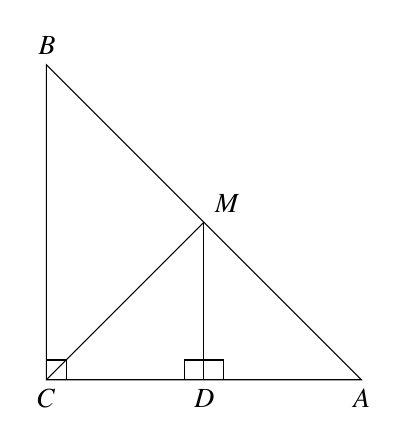
\begin{tikzpicture}
\coordinate (B) at (0,4);
\coordinate (A) at (4,0);
\coordinate (C) at (0,0);
\coordinate (D) at (2,0);
\coordinate (M) at (2,2);
\draw (A)node[below]{$A$}--(B)node[above]{$B$}--(C)node[below]{$C$}--cycle;
\draw(M)node[above right]{$M$}--(D)node[below]{$D$};
\draw(M)--(D);
\draw(M)--(C);
\tkzMarkRightAngle(B,C,A)
\tkzMarkRightAngle(A,D,M)
\tkzMarkRightAngle(C,D,M)
\end{tikzpicture}
}
\caption{Right Angled Triangle by Latex-Tikz}
\label{myfig}
\end{figure}
In $\triangle{ABC}$, $\vec{M}$ is midpoint of $\vec{AB}$ and $\vec{MD}$ is parallel to $\vec{BC}$, hence,
\begin{align}
&\vec{M} = \frac{\vec{A}+\vec{B}}{2}\label{eq1}\\
&\vec{MD} \parallel \vec{BC}\label{eq2}
\end{align}
As line drawn through mid point of one side of triangle parallel to other side bisects third side, hence proved from \eqref{eq1} and \eqref{eq2}, $\vec{D}$ is midpoint of $\vec{A}$ and $\vec{C}$ i.e
\begin{align}
&\vec{D} = \frac{\vec{A}+\vec{C}}{2}\label{eq3}
\end{align}
From figure \ref{myfig}, direction vectors of $\vec{MD}$ and  $\vec{AC}$ are given by,
\begin{align}
\vec{m_M_D} &= \vec{M}-\vec{D}\\
\implies\vec{m_M_D} &=\frac{\vec{A}+\vec{B}}{2} - \frac{\vec{A}+\vec{C}}{2}\\
\implies\vec{m_M_D}&=\frac{\vec{B}-\vec{C}}{2}\\ 
\vec{m_A_C} &= \vec{A}-\vec{C} 
\intertext{Hence,}
\vec{m_M_D}\vec{m_A_C} &=(\frac{\vec{B}-\vec{C}}{2})(\vec{A}-\vec{C})\\
\implies\vec{m_M_D}\vec{m_A_C} &=(\frac{\vec{m_B_C}}{2})(\vec{m_A_C})\\
\implies\vec{m_M_D}\vec{m_A_C}&=0\label{eq4}\quad{[$\because\vec{BC}\perp\vec{AC}$, $\angle{BCA}=90^{\circ}$]}
\end{align}
From \eqref{eq4}, it is proved that $\vec{MD}\perp\vec{AC}$\\
If $\vec{m_C_M}$, $\vec{m_C_D}$, $\vec{m_D_M}$, $\vec{m_A_D}$, $\vec{m_A_M}$ and $\vec{m_A_B}$ are direction vectors of $\vec{CM}$, $\vec{CD}$, $\vec{DM}$, $\vec{AD}$, $\vec{AM}$ and $\vec{AB}$ respectively then from the figure \ref{myfig}, after joining $\vec{M}$ and $\vec{C}$, in $\triangle{AMD}$ and $\triangle{CMD}$ we get,
\begin{align}
\vec{m_C_M} &= \vec{m_C_D}+\vec{m_D_M}\quad\text{[From $\triangle{CDM}]$}\\
\implies\vec{m_C_M} &= \vec{m_A_D}+\vec{m_D_M}\quad\text{[Proved in \eqref{eq3}]}\\
\implies\vec{m_C_M} &= \vec{m_A_M}\quad\text{[From $\triangle{ADM}$]}\\
\implies\vec{m_C_M} &= \vec{m_A_M} = \frac{\vec{m_A_B}}{2}\label{eqFinal}\quad\text{[From \eqref{eq1}]}
\end{align}
Hence proved, $\vec{CM}$ = $\vec{MA}$ = $\frac{1}{2}$ $\vec{AB}$
\end{document}